% Template for PLoS
% Version 3.4 January 2017
\documentclass[10pt,letterpaper]{article}
\usepackage[top=0.85in,left=2.75in,footskip=0.75in]{geometry}

% amsmath and amssymb packages, useful for mathematical formulas and symbols
\usepackage{amsmath,amssymb}

% Use adjustwidth environment to exceed column width (see example table in text)
\usepackage{changepage}

% Use Unicode characters when possible
\usepackage[utf8x]{inputenc}

% textcomp package and marvosym package for additional characters
\usepackage{textcomp,marvosym}

% cite package, to clean up citations in the main text. Do not remove.
% \usepackage{cite}

% Use nameref to cite supporting information files (see Supporting Information section for more info)
\usepackage{nameref,hyperref}

% line numbers
\usepackage[right]{lineno}

% ligatures disabled
\usepackage{microtype}
\DisableLigatures[f]{encoding = *, family = * }

% color can be used to apply background shading to table cells only
\usepackage[table]{xcolor}

% array package and thick rules for tables
\usepackage{array}

% create "+" rule type for thick vertical lines
\newcolumntype{+}{!{\vrule width 2pt}}

% create \thickcline for thick horizontal lines of variable length
\newlength\savedwidth
\newcommand\thickcline[1]{%
  \noalign{\global\savedwidth\arrayrulewidth\global\arrayrulewidth 2pt}%
  \cline{#1}%
  \noalign{\vskip\arrayrulewidth}%
  \noalign{\global\arrayrulewidth\savedwidth}%
}

% \thickhline command for thick horizontal lines that span the table
\newcommand\thickhline{\noalign{\global\savedwidth\arrayrulewidth\global\arrayrulewidth 2pt}%
\hline
\noalign{\global\arrayrulewidth\savedwidth}}


% Remove comment for double spacing
%\usepackage{setspace} 
%\doublespacing

% Text layout
\raggedright
\setlength{\parindent}{0.5cm}
\textwidth 5.25in 
\textheight 8.75in

% Bold the 'Figure #' in the caption and separate it from the title/caption with a period
% Captions will be left justified
\usepackage[aboveskip=1pt,labelfont=bf,labelsep=period,justification=raggedright,singlelinecheck=off]{caption}
\renewcommand{\figurename}{Fig}

% Use the PLoS provided BiBTeX style
% \bibliographystyle{plos2015}

% Remove brackets from numbering in List of References
\makeatletter
\renewcommand{\@biblabel}[1]{\quad#1.}
\makeatother

% Leave date blank
\date{}

% Header and Footer with logo
\usepackage{lastpage,fancyhdr,graphicx}
\usepackage{epstopdf}
\pagestyle{myheadings}
\pagestyle{fancy}
\fancyhf{}
\setlength{\headheight}{27.023pt}
\lhead{
\includegraphics[width=2.0in]{PLOS-submission.eps}}
\rfoot{\thepage/\pageref{LastPage}}
\renewcommand{\footrule}{\hrule height 2pt \vspace{2mm}}
\fancyheadoffset[L]{2.25in}
\fancyfootoffset[L]{2.25in}
\lfoot{\sf PLOS}

%% Include all macros below
\newcommand{\lorem}{{\bf LOREM}}
\newcommand{\ipsum}{{\bf IPSUM}}





\usepackage{forarray}
\usepackage{xstring}
\newcommand{\getIndex}[2]{
  \ForEach{,}{\IfEq{#1}{\thislevelitem}{\number\thislevelcount\ExitForEach}{}}{#2}
}

\setcounter{secnumdepth}{0}

\newcommand{\getAff}[1]{
  \getIndex{#1}{The George Washington University,IFPRI}
}

\providecommand{\tightlist}{%
  \setlength{\itemsep}{0pt}\setlength{\parskip}{0pt}}

\begin{document}
\vspace*{0.2in}

% Title must be 250 characters or less.
\begin{flushleft}
{\Large
\textbf\newline{Modeling impacts of drought on wheat and barley in Ethiopia} % Please use "sentence case" for title and headings (capitalize only the first word in a title (or heading), the first word in a subtitle (or subheading), and any proper nouns).
}
\newline
\\
Michael Mann\textsuperscript{\getAff{The George Washington University}}\textsuperscript{*},
James Warner\textsuperscript{\getAff{International Food Policy Research Institute}}\\
\bigskip
\textbf{\getAff{The George Washington University}}Department of Geography, Street, Washington, DC 20052\\
\textbf{\getAff{IFPRI}}Department, Street, Addis Abbaba, Ethiopia\\
\bigskip
* Corresponding author: mmann1123@gwu.edu\\
\end{flushleft}
% Please keep the abstract below 300 words
\section*{Abstract}
Lorem ipsum dolor sit amet, consectetur adipiscing elit. Curabitur eget
porta erat. Morbi consectetur est vel gravida pretium. Suspendisse ut
dui eu ante cursus gravida non sed sem. Nullam sapien tellus, commodo id
velit id, eleifend volutpat quam. Phasellus mauris velit, dapibus
finibus elementum vel, pulvinar non tellus. Nunc pellentesque pretium
diam, quis maximus dolor faucibus id. Nunc convallis sodales ante, ut
ullamcorper est egestas vitae. Nam sit amet enim ultrices, ultrices elit
pulvinar, volutpat risus.

% Please keep the Author Summary between 150 and 200 words
% Use first person. PLOS ONE authors please skip this step. 
% Author Summary not valid for PLOS ONE submissions.   
\section*{Author summary}
Lorem ipsum dolor sit amet, consectetur adipiscing elit. Curabitur eget
porta erat. Morbi consectetur est vel gravida pretium. Suspendisse ut
dui eu ante cursus gravida non sed sem. Nullam sapien tellus, commodo id
velit id, eleifend volutpat quam. Phasellus mauris velit, dapibus
finibus elementum vel, pulvinar non tellus. Nunc pellentesque pretium
diam, quis maximus dolor faucibus id. Nunc convallis sodales ante, ut
ullamcorper est egestas vitae. Nam sit amet enim ultrices, ultrices elit
pulvinar, volutpat risus.

\linenumbers

% Use "Eq" instead of "Equation" for equation citations.
\emph{Text based on plos sample manuscript, see
\url{http://journals.plos.org/ploscompbiol/s/latex}}

\section{Introduction}\label{introduction}

The ability to monitor and predict crop yields in developing countries
is critical to the successful adaptation to changes in our climate.
Increased temperatures and variability has already been linked to losses
in maize and wheat yields (-3.8 and 5.5\% respectively)and crop prices
globally {[}1{]}. Although much effort has been placed on modeling the
spatial distribution of these shifts, less effort has been placed on how
yields vary across space and time {[}2{]}. Advances in remote sensing
provide avenues to monitor agricultural crop health at high spatial and
temporal resolution. However, our ability to monitor changes in plant
productivity is still limited in the more complex environments common to
many developing countries {[}3{]}.

Remote sensing based efforts to characterize the extent, cultivation
practices, and productivity of global croplands has a long history. In
fact, agricultural monitoring motivated much of the earliest work in
remote sensing for example NASA's LACIE and AgRISTARS programs in the
1970s and 1980s and {[}4{]}). Since then, substantial progress has been
made in mapping cropland extent, crop types, irrigation status, cropping
intensity, and productivity from remotely sensed imagery. For example,
the MODIS Land Cover Product MCD12Q1 {[}8{]} provides operationally
produced, global scale maps of agriculture and agricultural-natural
mosaics at an annual time step and 500 m spatial resolution from
2001-present. A finer resolution (\textasciitilde{}30 m) dataset is
available for the conterminous United States which maps the annual
extent and type for over 250 crops using primarily Landsat imagery: the
Cropland Data Layer {[}{[}10{]}. These are but two prominent examples
out of a broad literature documenting a wide variety of efforts to map
cropland extent and type from remotely sensed imagery {[}11{]}. Remotely
sensed imagery has also been employed to map irrigated areas {[}17{]},
and cropping frequency/intensity {[}16{]}.

Initial efforts (e.g.~LACIE and AgRISTARS) primarily utilized remotely
sensed imagery to characterize the spatial extent and growth stage of
crops, but relied on models driven chiefly by meteorological information
to predict crop yield {[}21{]}. However, the biophysical link between
canopy spectral reflectance and net primary production has long been
established {[}23{]}; indicating that satellite measurements could play
a role in determining crop yield directly. Indeed, early experimental
work confirmed the usefulness of spectral measurements in predicting LAI
and intercepted PAR in crops {[}24{]}, a result that was later extended
to satellite measurements of spectral reflectance {[}27{]}. Spectral
measurements typically explain variability in LAI and intercepted PAR
better than crop yields because a variety of factors other than net
primary production (e.g.~weather during critical crop growth stages)
influence yield. Nevertheless, a wide number of studies have documented
highly explanatory empirical relationships between satellite measures
such as NDVI (in many forms: growing season maximum and mean, seasonally
integrated, etc.) and yields for a variety of crops, particularly at
regional scales {[}30{]}. Because certain crop growth stages are
particularly critical for final yield {[}36{]}, improved results are
often seen when remotely sensed data are used to characterize crop
phenology {[}37{]}. More recently, methods for forecasting yields with
remotely sensed variables at the field scale have been explored
{[}38{]}. In addition to establishing a direct relationship between
satellite measurements and crop yield, combining these observations with
model output, through formal or ad hoc data assimilation techniques has
also been demonstrated {[}40{]}.

The main objectives of this paper is to
\_\_\_\_\_\_\_\_\_\_\_\_\_\_\_\_\_. In particular, we will focus on the
application of \_\_\_\_\_\_\_\_\_\_\_\_\_\_\_\_\_\_\_. We also created
and present a suite of algorithms used to extract, summarize, and
organize remotely sensed data and prepare it for spatiotemporal
analysis.

\subsection{Drought meets
distribution}\label{drought-meets-distribution}

Spured by a long history of monsoon failures across the Sahel,
forecasters and aid teams axiciously watched eastern Africa at the onset
of a significant El Nino event in late 2014. Below average rainfalls in
2015-17 across the low lying pastoral communities and South Eastern
Ethiopia triggered an international effort to provide food aid to
roughly 8.5 million people in the summer of 2017 {[}43{]}. The
understated response from the Ethiopian government has lead to
accusations that the government is downplaying the severity of the
drought as early as 2016 {[}45{]}. Despite the reality of a severe and
crippling drought in food insecure low lying areas, there is little sign
of food shortages nationally, with a recent study observing no
significant change in grain prices throughout the country
((((\textbf{???})))). The lack of a price response would indicate that
while food insecure areas were hit heavily by water shortages largely
effecting livestock, leaving the highland areas largely unaffected or
triggering only minor losses. Despite international concern, conditions
up until the 2016-2017 growing season may have been largely handled by
domestic resources and trade flows, therefore requiring shifts in
distribution rather than a large-scale interational intervention.

Looking at the example of wheat production for the top 15 producing
zones (Figure: 1), we can see that total output has remained steady or
increased in the majority of top performing zones. This can be seen by
the increase in total production from 49,500 (?00s quintiles) in 2010 to
64,209 in the 2015 planting season. Additionally, we can see that the
total production of each zone (as indicated by the width of each bar)
generally increases over time, or remains relatively constant. Moreover
we can see that the rank of regions (as indicated by the plot order,
bottom being lowest rank, top being highest rank) remains surprisingly
steady dispite the exogenous shock of drought begining in the 2015
planing season.

\newpage

\emph{Figure 1: Total Wheat output of top 15 producing zones}

\texttt{r}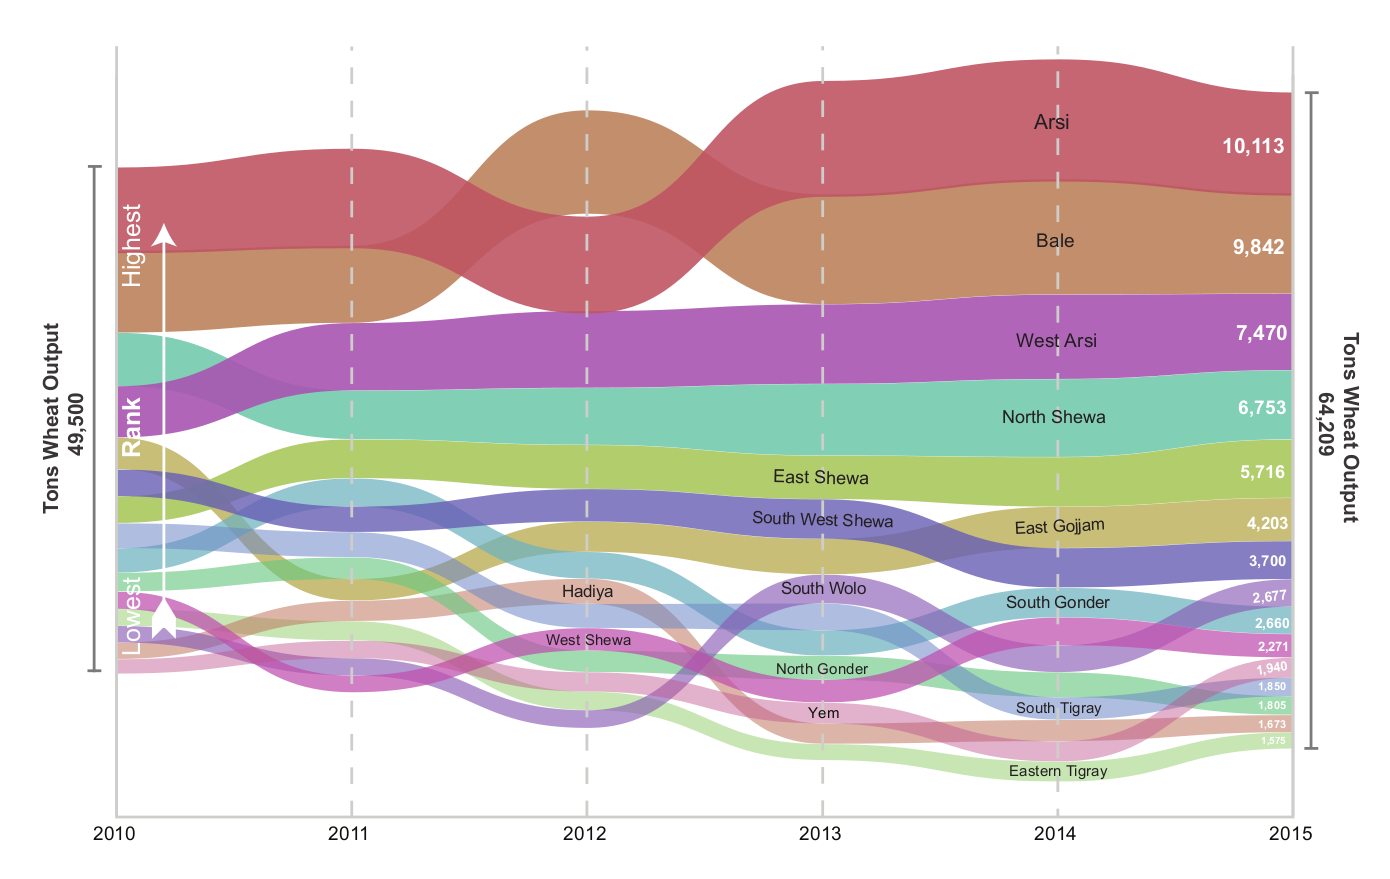
\includegraphics{/home/mmann1123/Documents/IFPRI_Ethiopia_Drought_2016/Visualizations/Wheat_Output_bottom40_rm_acd_v2.jpg}

We can see from Figure 2 three time series for the major regions
depicting the drought, in the top panel (a) the percentage of planted
area damaged by damage type, the middle panel (b) the percentage of area
planted in each major crop, in the bottom panel (c) median output per
hectare (OPH) in quintiles for each major crop. Although we see a marked
spike in reports of drought damage in the 2015 planting season (covering
harvest in 2016), we see a few important responses. First, we see that
although slight, farmers increased the percentage of area planted in
drought tolerant crops such as maize and sorghum. Second, we see that
although some regions saw declines in median output per hectare, these
losses are largely offset by gains in other crops or by the steady
increase in OPH since 2010.

\newpage

\emph{Figure 2: Drought in one graph }

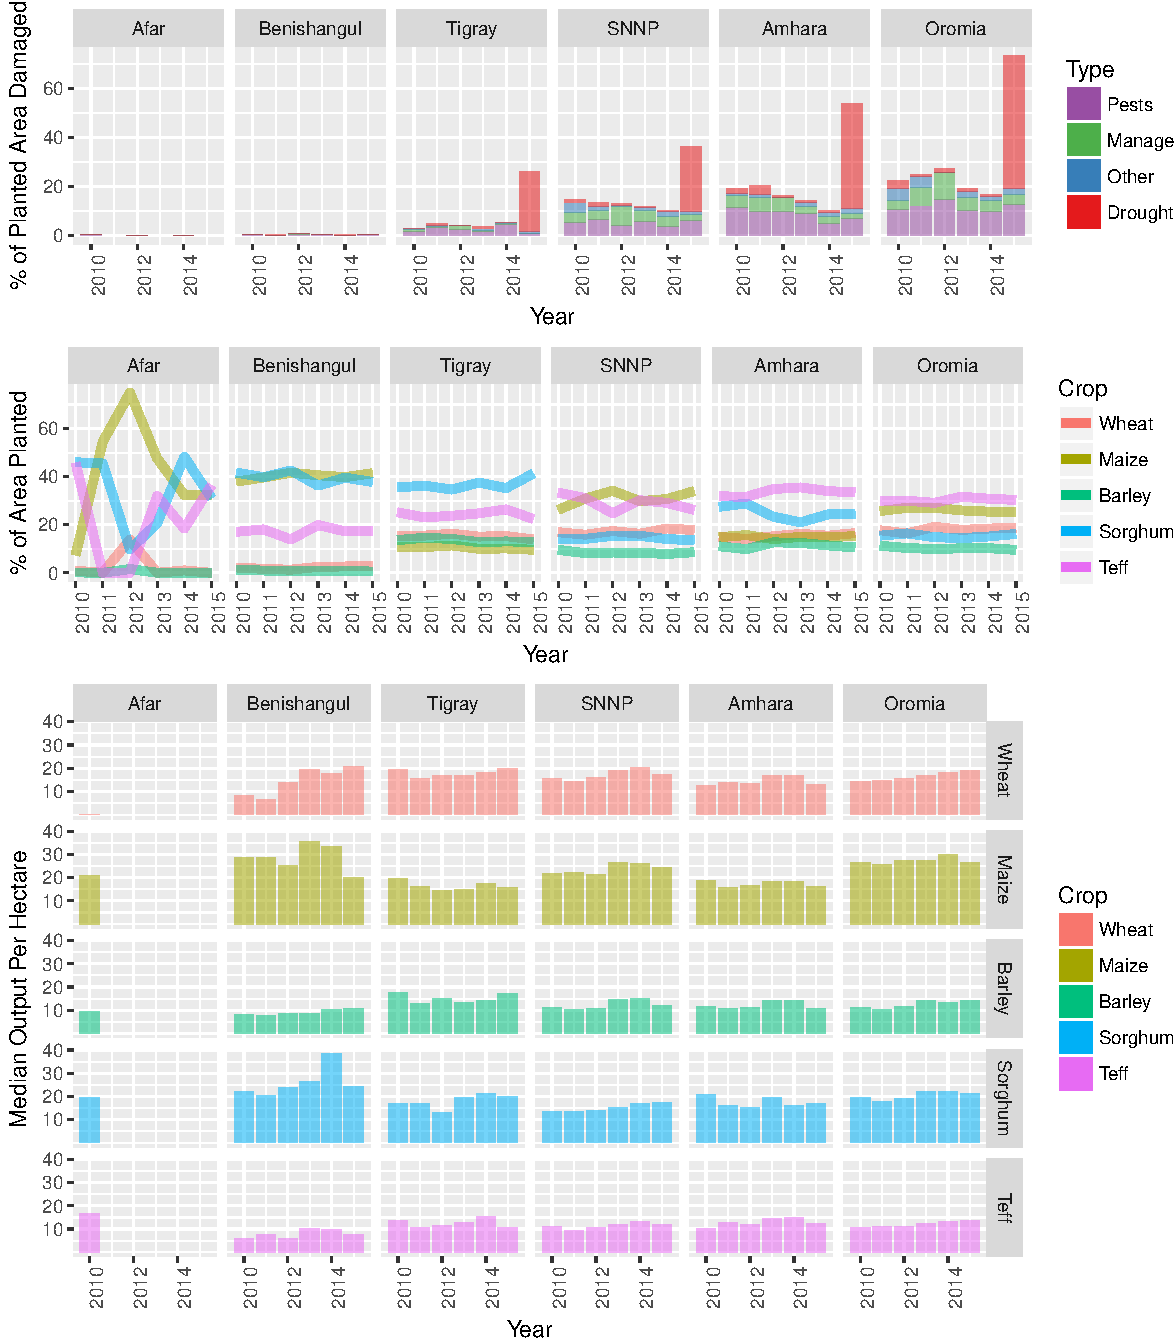
\includegraphics{IFPRI_2016_Report_Ethiopia_files/figure-latex/unnamed-chunk-2-1.pdf}

\pagebreak

\emph{Figure 3: Aggregate commodity trade flows }

\texttt{r}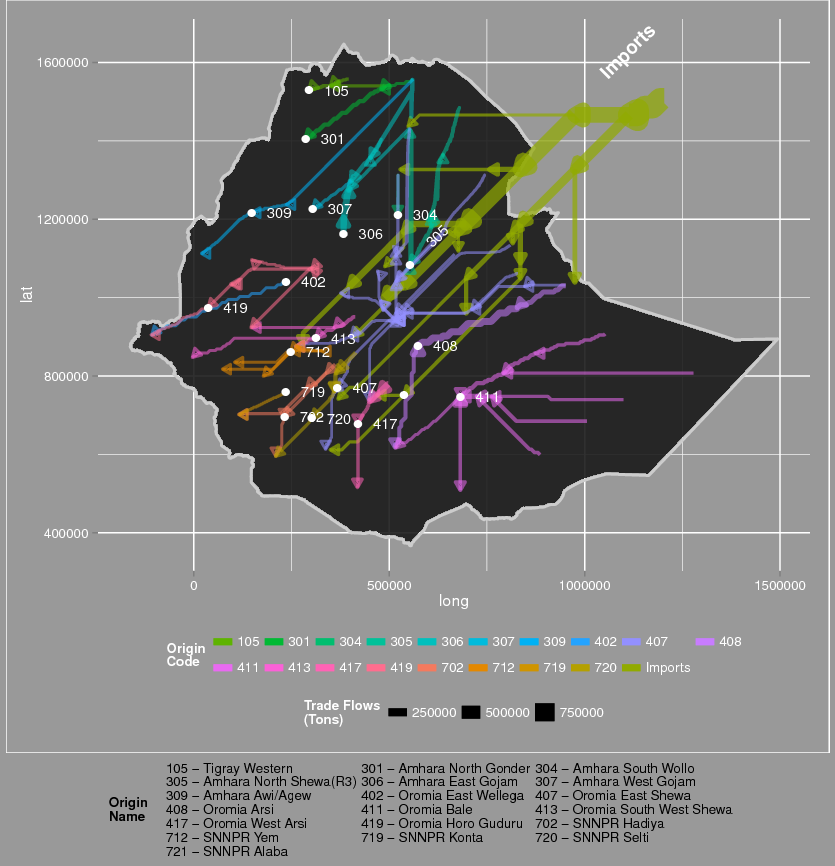
\includegraphics{/home/mmann1123/Documents/IFPRI_Ethiopia_Drought_2016/Writeup/ggplot_grey_legend_import_arrows3.png}

\section*{References}\label{references}
\addcontentsline{toc}{section}{References}

\hypertarget{refs}{}
\hypertarget{ref-Lobell616}{}
1. Lobell DB, Schlenker W, Costa-Roberts J. Climate trends and global
crop production since 1980. Science. American Association for the
Advancement of Science; 2011;333: 616--620.
doi:\href{https://doi.org/10.1126/science.1204531}{10.1126/science.1204531}

\hypertarget{ref-Ray2015}{}
2. Ray DK, Gerber JS, MacDonald GK, West PC. Climate variation explains
a third of global crop yield variability. Nature Communications. The
Author(s); 2015;6: 5989. Available:
\href{http://dx.doi.org/10.1038/ncomms6989\%20http://10.1038/ncomms6989\%20http://www.nature.com/articles/ncomms6989\%7B/\#\%7Dsupplementary-information}{http://dx.doi.org/10.1038/ncomms6989 http://10.1038/ncomms6989 http://www.nature.com/articles/ncomms6989\{\textbackslash{}\#\}supplementary-information}

\hypertarget{ref-Mann2015}{}
3. Mann ML, Warner J. Ethiopian Wheat Yield and Yield Gap Estimation: A
Small Area Integrated Data Approach. Addis Ababa, Ethiopia:
International Food Policy Research Institute; 2015.

\hypertarget{ref-macdonald1980global}{}
4. MacDonald RB, Hall FG. Global crop forecasting. Science. Washington;
1980;208: 670--679.

\hypertarget{ref-hatfield1983remote}{}
5. Hatfield J. Remote sensing estimators of potential and actual crop
yield. Remote Sensing of Environment. Elsevier; 1983;13: 301--311.

\hypertarget{ref-NASA1984}{}
6. NASA. AgRISTARS: Agriculture and resources inventory surveys through
aerospace remote sensing. technical report research report. AgRISTARS:
Agriculture and resources inventory surveys through aerospace remote
sensing. Technical Report Research Report. NASA; 1984.

\hypertarget{ref-pinter2003agricultural}{}
7. Pinter Jr PJ, Ritchie JC, Hatfield JL, Hart GF. The agricultural
research service's remote sensing program. Photogrammetric Engineering
\& Remote Sensing. American Society for Photogrammetry; Remote Sensing;
2003;69: 615--618.

\hypertarget{ref-friedl2002global}{}
8. Friedl MA, McIver DK, Hodges JC, Zhang X, Muchoney D, Strahler AH, et
al. Global land cover mapping from modis: Algorithms and early results.
Remote Sensing of Environment. Elsevier; 2002;83: 287--302.

\hypertarget{ref-friedl2010modis}{}
9. Friedl MA, Sulla-Menashe D, Tan B, Schneider A, Ramankutty N, Sibley
A, et al. MODIS collection 5 global land cover: Algorithm refinements
and characterization of new datasets. Remote sensing of Environment.
Elsevier; 2010;114: 168--182.

\hypertarget{ref-nass2003usda}{}
10. NASS U. USDA-national agricultural statistics service, cropland data
layer. United States Department of Agriculture, National Agricultural
Statistics Service, Marketing and Information Services Office,
Washington, DC {[}Available at http//nassgeodata gmu edu/Crop-Scape,
Last accessed September 2012{]}. 2003;

\hypertarget{ref-lobell2004cropland}{}
11. Lobell DB, Asner GP. Cropland distributions from temporal unmixing
of modis data. Remote Sensing of Environment. Elsevier; 2004;93:
412--422.

\hypertarget{ref-xiao2006mapping}{}
12. Xiao X, Boles S, Frolking S, Li C, Babu JY, Salas W, et al. Mapping
paddy rice agriculture in south and southeast asia using multi-temporal
modis images. Remote Sensing of Environment. Elsevier; 2006;100:
95--113.

\hypertarget{ref-thenkabail2007spectral}{}
13. Thenkabail P, GangadharaRao P, Biggs T, Krishna M, Turral H.
Spectral matching techniques to determine historical land-use/land-cover
(lulc) and irrigated areas using time-series 0.1-degree avhrr pathfinder
datasets. Photogrammetric Engineering \& Remote Sensing. 2007;73:
1029--1040.

\hypertarget{ref-ramankutty2008farming}{}
14. Ramankutty N, Evan AT, Monfreda C, Foley JA. Farming the planet: 1.
geographic distribution of global agricultural lands in the year 2000.
Global Biogeochemical Cycles. Wiley Online Library; 2008;22.

\hypertarget{ref-wardlow2008large}{}
15. Wardlow BD, Egbert SL. Large-area crop mapping using time-series
modis 250 m ndvi data: An assessment for the us central great plains.
Remote sensing of environment. Elsevier; 2008;112: 1096--1116.

\hypertarget{ref-biradar2011quantifying}{}
16. Biradar CM, Xiao X. Quantifying the area and spatial distribution of
double-and triple-cropping croplands in india with multi-temporal modis
imagery in 2005. International Journal of Remote Sensing. Taylor \&
Francis; 2011;32: 367--386.

\hypertarget{ref-thenkabail2009global}{}
17. Thenkabail PS, Biradar CM, Noojipady P, Dheeravath V, Li Y, Velpuri
M, et al. Global irrigated area map (giam), derived from remote sensing,
for the end of the last millennium. International Journal of Remote
Sensing. Taylor \& Francis; 2009;30: 3679--3733.

\hypertarget{ref-portmann2010mirca2000}{}
18. Portmann FT, Siebert S, Döll P. MIRCA2000---Global monthly irrigated
and rainfed crop areas around the year 2000: A new high-resolution data
set for agricultural and hydrological modeling. Global Biogeochemical
Cycles. Wiley Online Library; 2010;24.

\hypertarget{ref-gray2014mapping}{}
19. Gray J, Friedl M, Frolking S, Ramankutty N, Nelson A, Gumma MK.
Mapping asian cropping intensity with modis. IEEE Journal of Selected
Topics in Applied Earth Observations and Remote Sensing. IEEE; 2014;7:
3373--3379.

\hypertarget{ref-li2014mapping}{}
20. Li L, Friedl MA, Xin Q, Gray J, Pan Y, Frolking S. Mapping crop
cycles in china using modis-evi time series. Remote Sensing.
Multidisciplinary Digital Publishing Institute; 2014;6: 2473--2493.

\hypertarget{ref-idso1977remote}{}
21. Idso SB, Jackson RD, Reginato RJ. Remote-sensing of crop yields.
Science. American Association for the Advancement of Science; 1977;196:
19--25.

\hypertarget{ref-doraiswamy2003crop}{}
22. Doraiswamy PC, Moulin S, Cook PW, Stern A. Crop yield assessment
from remote sensing. Photogrammetric engineering \& remote sensing.
American Society for Photogrammetry; Remote Sensing; 2003;69: 665--674.

\hypertarget{ref-tucker1986satellite}{}
23. Tucker C, Sellers P. Satellite remote sensing of primary production.
International journal of remote sensing. Taylor \& Francis; 1986;7:
1395--1416.

\hypertarget{ref-daughtry1983spectral}{}
24. Daughtry C, Gallo K, Bauer ME. Spectral estimates of solar radiation
intercepted by corn canopies. Agronomy Journal. American Society of
Agronomy; 1983;75: 527--531.

\hypertarget{ref-asrar1984estimating}{}
25. Asrar G, Fuchs M, Kanemasu E, Hatfield J. Estimating absorbed
photosynthetic radiation and leaf area index from spectral reflectance
in wheat. Agronomy journal. American Society of Agronomy; 1984;76:
300--306.

\hypertarget{ref-clevers1997simplified}{}
26. Clevers J. A simplified approach for yield prediction of sugar beet
based on optical remote sensing data. Remote Sensing of Environment.
Elsevier; 1997;61: 221--228.

\hypertarget{ref-tucker1980relationship}{}
27. Tucker C, Holben B, Elgin Jr J, McMurtrey III J, others.
Relationship of spectral data to grain yield variation. Photogrammetric
Engineering and Remote Sensing. 1980;46: 657--666.

\hypertarget{ref-groten1993ndvi}{}
28. Groten S. NDVI---crop monitoring and early yield assessment of
burkina faso. TitleREMOTE SENSING. Taylor \& Francis; 1993;14:
1495--1515.

\hypertarget{ref-bartholome1988radiometric}{}
29. Bartholome E. Radiometric measurements and crop yield forecasting
some observations over millet and sorghum experimental plots in mali.
International journal of remote sensing. Taylor \& Francis; 1988;9:
1539--1552.

\hypertarget{ref-rasmussen1992assessment}{}
30. Rasmussen MS. Assessment of millet yields and production in northern
burkina faso using integrated ndvi from the avhrr. International Journal
of Remote Sensing. Taylor \& Francis; 1992;13: 3431--3442.

\hypertarget{ref-benedetti1993use}{}
31. Benedetti R, Rossini P. On the use of ndvi profiles as a tool for
agricultural statistics: The case study of wheat yield estimate and
forecast in emilia romagna. Remote Sensing of Environment. Elsevier;
1993;45: 311--326.

\hypertarget{ref-funk2009phenologically}{}
32. Funk C, Budde ME. Phenologically-tuned modis ndvi-based production
anomaly estimates for zimbabwe. Remote Sensing of Environment. Elsevier;
2009;113: 115--125.

\hypertarget{ref-becker2010generalized}{}
33. Becker-Reshef I, Vermote E, Lindeman M, Justice C. A generalized
regression-based model for forecasting winter wheat yields in kansas and
ukraine using modis data. Remote Sensing of Environment. Elsevier;
2010;114: 1312--1323.

\hypertarget{ref-becker2010monitoring}{}
34. Becker-Reshef I, Justice C, Sullivan M, Vermote E, Tucker C, Anyamba
A, et al. Monitoring global croplands with coarse resolution earth
observations: The global agriculture monitoring (glam) project. Remote
Sensing. Molecular Diversity Preservation International; 2010;2:
1589--1609.

\hypertarget{ref-mkhabela2011crop}{}
35. Mkhabela M, Bullock P, Raj S, Wang S, Yang Y. Crop yield forecasting
on the canadian prairies using modis ndvi data. Agricultural and Forest
Meteorology. Elsevier; 2011;151: 385--393.

\hypertarget{ref-butler2015variations}{}
36. Butler EE, Huybers P. Variations in the sensitivity of us maize
yield to extreme temperatures by region and growth phase. Environmental
Research Letters. IOP Publishing; 2015;10: 034009.

\hypertarget{ref-bolton2013forecasting}{}
37. Bolton DK, Friedl MA. Forecasting crop yield using remotely sensed
vegetation indices and crop phenology metrics. Agricultural and Forest
Meteorology. Elsevier; 2013;173: 74--84.

\hypertarget{ref-lobell2015scalable}{}
38. Lobell DB, Thau D, Seifert C, Engle E, Little B. A scalable
satellite-based crop yield mapper. Remote Sensing of Environment.
Elsevier; 2015;164: 324--333.

\hypertarget{ref-gao2017toward}{}
39. Gao F, Anderson MC, Zhang X, Yang Z, Alfieri JG, Kustas WP, et al.
Toward mapping crop progress at field scales through fusion of landsat
and modis imagery. Remote Sensing of Environment. Elsevier; 2017;188:
9--25.

\hypertarget{ref-mo2005prediction}{}
40. Mo X, Liu S, Lin Z, Xu Y, Xiang Y, McVicar T. Prediction of crop
yield, water consumption and water use efficiency with a svat-crop
growth model using remotely sensed data on the north china plain.
Ecological Modelling. Elsevier; 2005;183: 301--322.

\hypertarget{ref-moriondo2007simple}{}
41. Moriondo M, Maselli F, Bindi M. A simple model of regional wheat
yield based on ndvi data. European Journal of Agronomy. Elsevier;
2007;26: 266--274.

\hypertarget{ref-de2007crop}{}
42. De Wit A de, Van Diepen C. Crop model data assimilation with the
ensemble kalman filter for improving regional crop yield forecasts.
Agricultural and Forest Meteorology. Elsevier; 2007;146: 38--56.

\hypertarget{ref-reliefweb2017}{}
43. Ethiopia: Drought - 2015-2017 {[}Internet{]}. ReliefWeb. Available:
\url{https://reliefweb.int/disaster/dr-2015-000109-eth}

\hypertarget{ref-reliefweb_2017b}{}
44. Mid-year review, ethiopia humanitarian requirements document, july
2017 {[}Internet{]}. ReliefWeb. 2017. Available:
\url{https://reliefweb.int/report/ethiopia/mid-year-review-ethiopia-humanitarian-requirements-document-july-2017}

\hypertarget{ref-schemm_2016}{}
45. Schemm P. Ethiopia is facing a devastating drought, and food aid may
soon run out {[}Internet{]}. The Washington Post. WP Company; 2016.
Available:
\url{http://www.washingtonpost.com/sf/world/2016/02/22/history-repeats-itself-in-ethiopia/?utm_term=.2b7bb38f3a3e}

\hypertarget{ref-schemm_2017}{}
46. Schemm P. Ethiopia is facing a killer drought. but it's going almost
unnoticed. {[}Internet{]}. The Washington Post. WP Company; 2017.
Available:
\url{https://www.washingtonpost.com/news/worldviews/wp/2017/05/01/ethiopia-is-facing-a-killer-drought-but-its-going-almost-unnoticed/?utm_term=.ad44d46b0631}

\nolinenumbers


\end{document}

